\subsection{SOCKS 5}

Protocolul SOCKS este folosit pentru a crea conexiuni TCP către destinații arbitrare folosind un proxy.
În ultima versiune standardizată a protocolului (versiunea 5), durează doua RTT-uri (sau 3, dacă se face și autentificare) până când datele pot circula între client și server.

\begin{figure}[h]
	\centering
	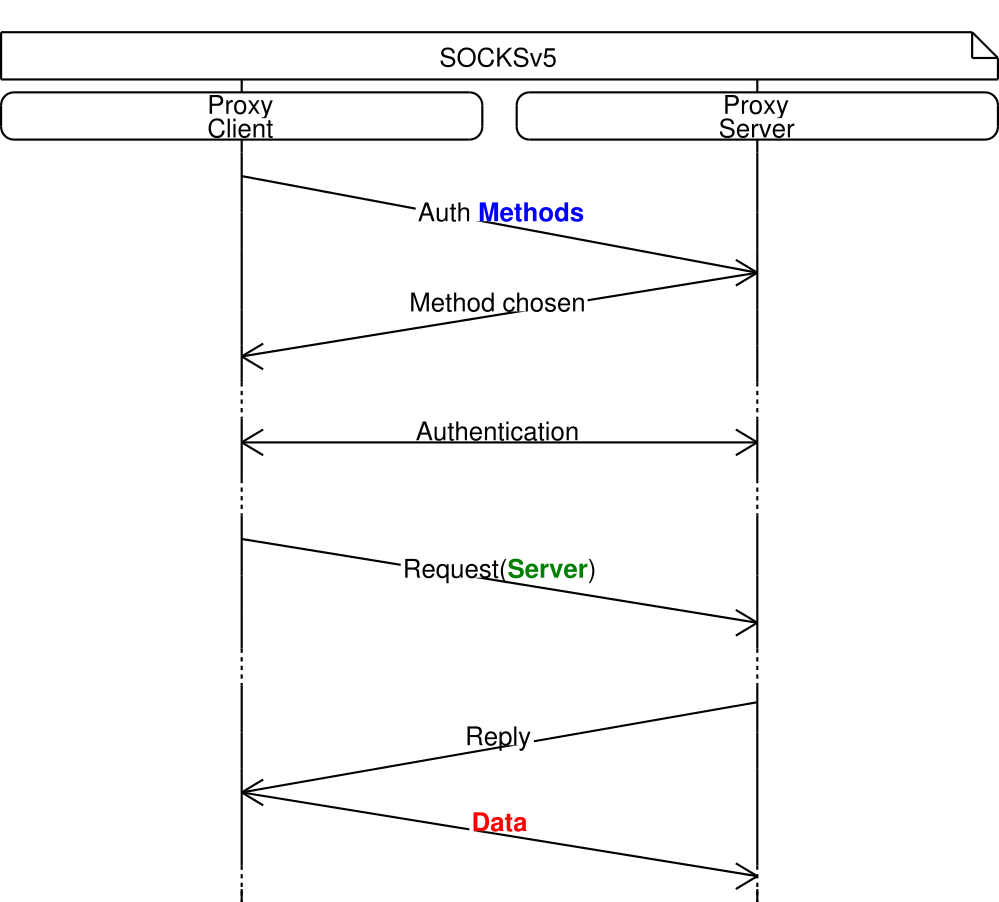
\includegraphics[scale=0.7]{figures/socks/socks5op.png}
	\caption{Mod de operare SOCKS 5}
    	\label{fig:socks5op}
\end{figure}

In SOCKS 5 (versiunea curentă a protocolului, v. fig \ref{fig:socks5op}), clientul deschide o conexiune căte proxy si parcurge urmatoarele etape înainte să transmită date către server:
\begin{itemize}
	\item Negocierea metodei de autentificare (1 RTT): Clientul trimite un mesaj care conține metodele de autentificare suportate. Proxy-ul răspunde cu metoda de autentificare aleasă.
	\item Autentificarea propriu-zisă (0-1 RTT-uri): Acest pas poate să lipsească, dacă nu se face autentificare. Altfel, durează tipic un RTT.
	\item Crearea socket-ului (1 RTT): Clientul trimite adresa și portul server-ului la care vrea sa se conecteze. Proxy-ul încearcă să onoreze cererea clientului și îi trimite un răspuns cu rezultatul.
\end{itemize}


\subsection{SOCKS 6}

Am dezvoltat versiunea 6 a protocolului SOCKS, pe care o propunem pentru standardizare în cadrul IETF. Momentan se află in starea de Internet Draft~\cite{socks6}.
Principalele îmbunătățiri introduse în această versiune sunt:
\begin{itemize}
	\item Clientul are un comportament optimist și trimite cât mai multe informații către proxy, fără a aștepta să se termine autentificarea.
	\item Semanticile cererilor imită semanticile TCP Fast Open~\cite{rfc7413}. În cerere, clientul poate include și potențialul payload pentru SYN-ul inițial trimis către server.
	\item Protocolul poate fi extins folosind opțiuni, similare cu opțiunile TCP.
	\item Folosint opțiunile menționate mai sus, se pot implementa scheme de autentificare în 0 RTT-uri.
\end{itemize}


\begin{figure}[h]
	\centering
	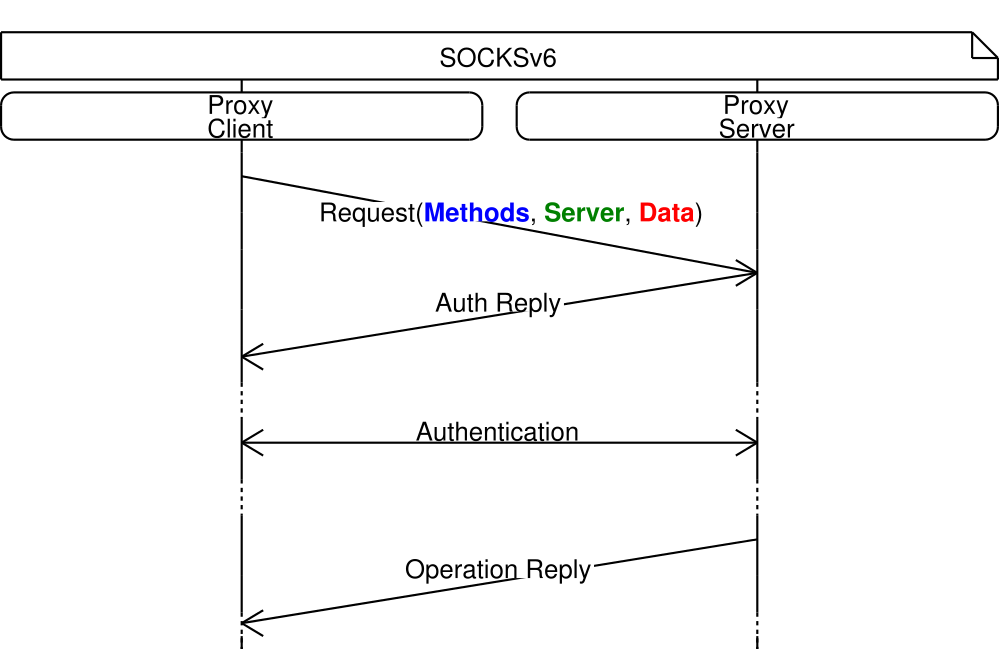
\includegraphics[scale=0.7]{figures/socks/socks6op1st.png}
	\caption{Mod de operare SOCKS 6 (prima conexiune cu autentificare)}
    	\label{fig:socks6op1st}
\end{figure}

\begin{figure}[h]
	\centering
	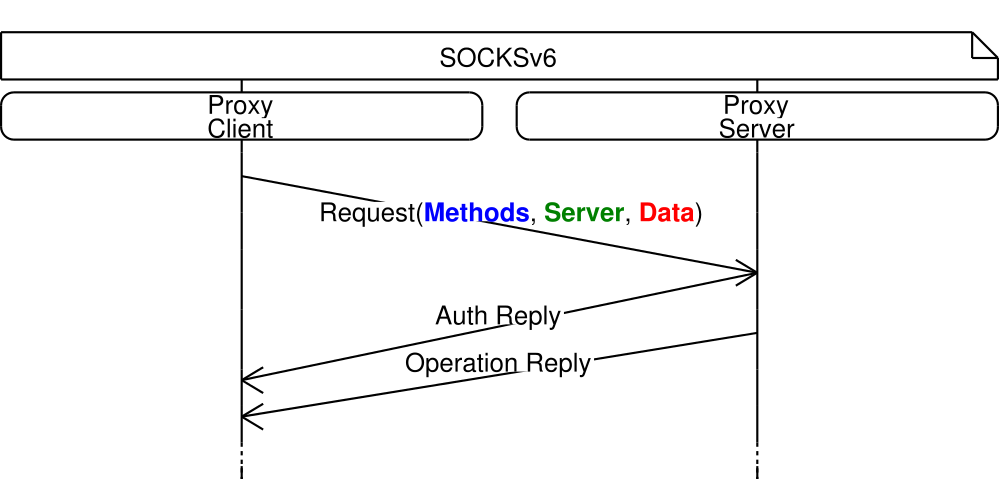
\includegraphics[scale=0.7]{figures/socks/socks6op2nd.png}
	\caption{Mod de operare SOCKS 6 (conexiuni ulterioare)}
    	\label{fig:socks6op2nd}
\end{figure}

Atunci când un client SOCKS 6 încearcă să se conecteze la un server, deschide o conexiune către un proxy (v. fig. \ref{fig:socks6op1st}) .
Clientul începe prin a trimite o cerere (SOCKS Request), care conține, printre altele:
\begin{itemize}
	\item Metodele de autentificare cunoscute de client.
	\item Adresa și portul server-ului.
	\item Primii octeți din fluxul de date destinat server-ului.
\end{itemize}

Proxy-ul răspunde cu un Authentication reply, care indică protocolul de autentificare care trebuie folosit.
Apoi se execută protocolul de autentificare ales, lucru care poate dura un RTT sau mai mult.

Dacă autentificarea s-a terminat cu succes, proxy-ul încearcă să creeze conexiunea cerută de client, si trimite un Operation Reply, care indică dacă s-a putut realiza conexiunea sau nu.

În cererile ulterioare, clientul poate să includă date de autentificare in cerere (Request), lucru care îl scutește de etapa de autentificare (fig. \ref{fig:socks6op1st}).
Astfel, se poate obține un răspuns de la server intr-un singur RTT, cu 2-3 RTT-uri mai rapid decât cu SOCKS 5.

